\info{
	Il est conseillé de se référer aux tableaux [Notations-Spécifique au stage]
	et \ref{tab:model} pour la signification des notations déjà introduites et utilisées dans ce chapitre.
}

\subsection{Nombre de simulations}
\label{subsec:nb-simulations}

Afin d'étudier la relation entre le $\Delta$ optimum et différentes quantités caractéristiques aux données, on va effectuer une simulation de Monte-Carlo.

On décide de générer $\mathsf{mc} = 200$ simulations de Monte-Carlo, afin d'obtenir les résultats les plus robustes possibles pour l'estimation du risque $\esperance{\distnorme 2 {\widehat \Theta} {\widetilde \Theta}}$\footnote{le raisonnement pour le choix du risque utilisé sera explicité en section \ref{sec:choix_risque_couple}}, tout en gardant un temps de calcul raisonnable. On fait varier $\lambda$ de $30$ à $480$ en incrémentant de $15$ à chaque fois. L'idée et de pouvoir regarder si il existe une relation entre $\Delta^*$ et la position du nombre moyen de points observés par courbe $(\lambda)$ par rapport au nombre de courbes $(N)$.

\smallskip

\noindent Il est possible de voir comment les paramètres que l'on va définir sont utilisés dans l'implémentation en annexe \ref{annexe:code}.


\newcommand{\tlnm}{T^{[\lambda]}_{n}[m]}
\newcommand{\mset}{\llbracket 1, M_n \rrbracket}
\newcommand{\nset}{\llbracket 1, N \rrbracket}
\newcommand{\lbdset}{\llbracket 30, 45, \dots , 480 \rrbracket}
\newcommand{\genxset}{\bigl(\tlnm, X_n(\tlnm)\bigr)_{m \in \mset}}
\newcommand{\simset}{\left\{ \genxset \, : \, n \in \nset, \, \lambda \& N \textsf{ fixés } \right\}}
\newcommand{\simsetall}{\left\{ \genxset \, : \, N \in \overrightarrow N, \, \lambda \in \lbdset, \, n \in \nset \right\}}


\subsection{Fonction de Hurst}
\label{sec:sim_fcn_hurst}
\begin{minipage}{0.47\linewidth}
	On appelle $H : t \mapsto H_t$ la fonction de Hurst. Celle qui a été choisie est la suivante :

	\begin{equation*}
		H^{[h_l, h_r, s, pos]}_{\textsf{logistic}} : \begin{array}{ccc}
			[0,1] & \longrightarrow & [h_l, h_r]
			\\
			t     & \longmapsto     & h_l + \frac{(h_r - h_l)}{1 + e^{-s(t - pos)}}
		\end{array}
	\end{equation*}

	La fonction de Hurst retenue est la suivante :

	\begin{equation*}
		H^{[0.4, 0.8, 5, 0.5]}_{\textsf{logistic}}
	\end{equation*}

	On dispose donc d'une régularité locale qui varie sur $\mathcal T$, tout en ayant une évolution pas trop brusque. Nous allons étudier le comportement du $\Delta$ lors de l'estimation de la régularité locale en les points suivants :

	\begin{equation*}
		\vec t = \begin{bmatrix} 0.3 \\ 0.4 \\ 0.5 \\ 0.6 \\ 0.7 \\ 0.8 \end{bmatrix}
		\quad\quad
		H(\, \vec t \,) =
		\begin{bmatrix}
			0.51 \\ 0.55 \\ 0.6 \\ 0.65 \\ 0.69 \\ 0.73
		\end{bmatrix}
	\end{equation*}

\end{minipage}
\hfill
\begin{minipage}{0.47\linewidth}
	\begin{figure}[H]
		\centering
		\begin{tikzpicture}
			\begin{axis}[
					width=\textwidth,
					xlabel=$t$,
					ylabel={$H^{[0.4, 0.8, 5, 0.5]}_{\textsf{logistic}}(t)$},
					xmin=0, xmax=1,
					ymin=0.4, ymax=0.8,
					axis lines=center,
					axis on top=true,
					domain=0:1,
					samples=100,
					legend style={at={(0.5,-0.15)},anchor=north},
					legend entries={Fonction de Hurst, Points d'estimation de la régularité locale},
				]
				\addplot [mark=none,smooth,blue] {0.4 + (0.8 - 0.4)/(1 + exp(-5*(x - 0.5)))};
				\addplot [only marks,mark=*] coordinates {
						(0.3,0.51)
						(0.4,0.55)
						(0.5,0.6)
						(0.6,0.65)
						(0.7,0.69)
						(0.8,0.73)
					};
			\end{axis}
		\end{tikzpicture}
		\caption{Hurst Function: Logistic}
		\label{plot:hurst-logistic}
	\end{figure}
\end{minipage}


\subsection{Constante de Hölder}
\label{subsec:constante-holder}

On décide de simuler des mouvements browniens multi-fractionnaires de constante de Hölder $L_t$ identique sur tout le support. (\edited on se concentre sur l'estimation de $H$)
\begin{equation*}
	\forall t \quad L_t = 1
\end{equation*}



\subsection{Moyenne}
\label{subsec:moyenne}
\begin{minipage}{0.47\linewidth}
	On appelle $H : t \mapsto H_t$ la fonction de Hurst. Celle qui a été choisie est la suivante :

	\begin{equation*}
		H^{[h_l, h_r, s, pos]}_{\textsf{logistic}} : \begin{array}{ccc}
			[0,1] & \longrightarrow & [h_l, h_r]
			\\
			t     & \longmapsto     & h_l + \frac{(h_r - h_l)}{1 + e^{-s(t - pos)}}
		\end{array}
	\end{equation*}

	La fonction de Hurst retenue est la suivante :

	\begin{equation*}
		H^{[0.4, 0.8, 5, 0.5]}_{\textsf{logistic}}
	\end{equation*}

	On dispose donc d'une régularité locale qui varie sur $\mathcal T$, tout en ayant une évolution pas trop brusque. Nous allons étudier le comportement du $\Delta$ lors de l'estimation de la régularité locale en les points suivants :

	\begin{equation*}
		\vec t = \begin{bmatrix} 0.3 \\ 0.4 \\ 0.5 \\ 0.6 \\ 0.7 \\ 0.8 \end{bmatrix}
		\quad\quad
		H(\, \vec t \,) =
		\begin{bmatrix}
			0.51 \\ 0.55 \\ 0.6 \\ 0.65 \\ 0.69 \\ 0.73
		\end{bmatrix}
	\end{equation*}

\end{minipage}
\hfill
\begin{minipage}{0.47\linewidth}
	\begin{figure}[H]
		\centering
		\begin{tikzpicture}
			\begin{axis}[
					width=\textwidth,
					xlabel=$t$,
					ylabel={$H^{[0.4, 0.8, 5, 0.5]}_{\textsf{logistic}}(t)$},
					xmin=0, xmax=1,
					ymin=0.4, ymax=0.8,
					axis lines=center,
					axis on top=true,
					domain=0:1,
					samples=100,
					legend style={at={(0.5,-0.15)},anchor=north},
					legend entries={Fonction de Hurst, Points d'estimation de la régularité locale},
				]
				\addplot [mark=none,smooth,blue] {0.4 + (0.8 - 0.4)/(1 + exp(-5*(x - 0.5)))};
				\addplot [only marks,mark=*] coordinates {
						(0.3,0.51)
						(0.4,0.55)
						(0.5,0.6)
						(0.6,0.65)
						(0.7,0.69)
						(0.8,0.73)
					};
			\end{axis}
		\end{tikzpicture}
		\caption{Hurst Function: Logistic}
		\label{plot:hurst-logistic}
	\end{figure}
\end{minipage}


\subsection{Noyau de la relation FAR(1)}
\label{subsec:noyau-far}
\begin{minipage}{0.48\linewidth}
	On décide de simuler un FAR(1) basé sur un opérateur linéaire intégral :

	\begin{equation*}
		X_{n+1} = \phi(X_n) + \varepsilon_{n+1}
	\end{equation*}

	avec : $\phi : f \mapsto \displaystyle\int_{\mathcal T} f(u) \beta(u, \cdot \,) \, du$

	C'est une modélisation fréquente des FAR(1). Le noyaux que l'on considère dans l'opérateur intégral pour les simulations est le suivant :


	\begin{equation*}
		\beta : \, \begin{array}{ccc}
			[0,1]^2 & \longrightarrow & \mathbb R
			\\
			(t,s)   & \longmapsto     & \frac 9 4 t\sqrt{ s(1-s) }
		\end{array}
	\end{equation*}

\end{minipage}
\hfill
\begin{minipage}{0.48\linewidth}
	\begin{figure}[H]
		\centering
		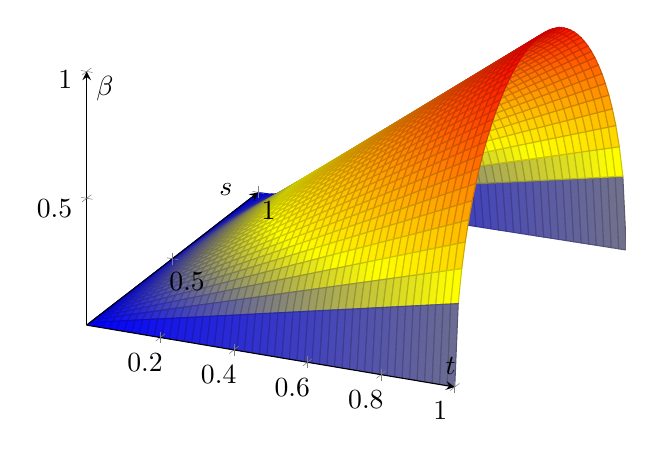
\begin{tikzpicture}
			\begin{axis}[
					xlabel=$t$,
					ylabel=$s$,
					zlabel=$\beta$,
					xmin=0, xmax=1,
					ymin=0, ymax=1,
					zmin=0, zmax=1,
					axis lines=center,
					axis on top=true,
					domain=0:1,
					samples=50,
				]
				\addplot3 [surf] {9/4*x*sqrt(y*(1-y))};
			\end{axis}
		\end{tikzpicture}
		\caption{Graphique du noyau intégral pour la relation FAR(1)}
		\label{graph:far_kernel}
	\end{figure}
\end{minipage}

\bigskip

On notera que le noyaux utilisé pour la relation de $\operatorname{FAR}(1)$ est une fonction lisse. Ainsi il remplit aisément la condition pour que le $\operatorname{FAR}(1)$ hérite de la régularité du mouvement brownien multi-fractionnaire généré.


\subsection{Nombre de courbes}
\label{subsec:nb-courbes}
Afin d'étudier le lien potentiel qu'il pourrait y avoir entre le nombre de courbes observées et le $\Delta$ optimal pour l'estimation de la régularité locale, on choisit plusieurs valeurs de nombres de courbes observées de telle sorte à avoir un \og petit \fg et un \og grand \fg nombre de courbes observées.

On choisit les valeurs suivantes concernant le nombre de courbes observées :

\begin{equation*}
	\vec N = [ 100, 200, 300, 400]
\end{equation*}

Ainsi on traîte les cas de ce qu'on pourrait considérer comme la limite avant d'entrer dans un cas \og sparse \fg (en terme du nombre d'observations de courbe), jusqu'à un nombre de courbe que l'on peut considérer important.

\subsection{Nombre moyen de points observés par courbe}
\label{subsec:nb-moy-pts-obs-par-courbe}
Le nombre de points observés sur la courbe $X_n$ est défini comme étant la variable aléatoire $M_n$. Dans le cadre de notre simulation, $M_n$ suit une loi de poisson de paramètre $\lambda$. Ainsi, $\esperance{M_n} = \lambda$ dans le cadre de notre simulation.

On effectue donc une simulation d'un échantillon de série temporelle $\operatorname{FAR}(1)$ par nombre moyen de points que l'on souhaite observer sur les courbes ($\lambda$). Afin de traîter différents cas, d'observation \og dense \fg à observation \og sparse \fg (dans le sens du nombre de points par courbe), on fait varier $\lambda$ de $30$ points par courbe en moyenne à $480$ points. L'idée est de voir ensuite si il y a une relation entre le $\Delta^*$ et le fait que l'on ait $\lambda$ petit, similaire ou grand par rapport à $N$.

\subsection{Ensemble des $\Delta$ testés}
\label{subsec:delta-test}

On souhaite obtenir plusieurs graphiques avec $\Delta$ sur l'axe des abscisses afin de pouvoir étudier le comportement de diverses quantitées, dont le risque euclidien, lorsque l'on fait varier $\Delta$ avec certains paramètres fixés (nombre de courbes observées, nombre moyen de points observés par courbe, ...). Toutefois plus on va considérer de $\Delta$, et plus la simulation sera coûteuse. En effet, on a vu en section \ref{rem:inversion_matrice_covariance_mfbm_informel} que l'odre de complexité de la simulation du mfBm est de $\mathcal O \bigl( \operatorname{card} \mathds T^3 \bigr)$, avec $\mathds T$ les points où l'on doit évaluer nos $\famfinie X 1 n$. Dans notre cas, le nombre de points considérés pour la simulation est :

\begin{equation*}
	\underbracket[0.187ex]{\dim \vec\Delta}_{30} \times \underbracket[0.187ex]{3}_{t_1 / t_2 / t_3} \times \underbracket[0.187ex]{\dim \vec t}_{6} + \underbracket[0.187ex]{n_{Grid\_\int}}_{100} + \underbracket[0.187ex]{\lambda}_{\leq 480} \leq \underbracket[0.187ex]{640}_{fixe} + \underbracket[0.187ex]{480}_{pts \, aleat} = 1 \, 120
\end{equation*}

Pour assurer un équilibre entre le nombre de points et les temps de simulation, nous choisissons 30 valeurs uniformément réparties entre 0.01 et 0.2 pour $\Delta$. Au-delà de cette plage, la largeur des intervalles pour l'évaluation de la régularité devient disproportionnée par rapport à la taille du support, rendant inappropriée la notion de \og régularité locale \fg.

\begin{equation*}
	\vec \Delta = \left[ 0.01 \cdots  0.2 \right]_{30}
\end{equation*}


\subsection{Bruit blanc}
\label{subsec:bruit-blanc}

Une fois que l'on a simulé :

\begin{equation*}
	\famfinie X 1 n \quad \textsf{vérifiant} \quad X_{n+1} = \phi(X_n) + \xi_n
\end{equation*}

on doit désormais reproduire l'erreur de mesure, pour cela chaque courbe est ensuite bruitée en rajoutant un bruit blanc :

\begin{equation*}
	\eta \sim \mathcal N ( 0, 0.04 )
\end{equation*}

Il est important d'avoir un bruit blanc d'écart type d'un ordre de grandeur en dessous de celui des valeurs prises par le processus, sinon l'estimation serait mauvaise quoi qu'il arrive. En effet le bruit écraserait à lui tout seul toute l'information fine de régularité.


\subsection{Résumé des Paramètres}
\label{subsec:resume-params-simul}

\begin{table}[H]
	\centering
	\begin{tabular}{l|l|ll|l|}
		\cline{2-5}
		\textbf{}                                                                  & \textbf{nombre de valeurs testées} & \multicolumn{1}{l|}{\textbf{de}} & \textbf{jusqu'à}         & \textbf{valeur}          \\ \hline
		\multicolumn{1}{|l|}{\textit{\textbf{$\Delta$}}}                           & $30$                               & $0.01$                           & $0.2$                    & \cellcolor[HTML]{C0C0C0} \\
		\multicolumn{1}{|l|}{\textit{\textbf{$\lambda$}}}                          & $30$                               & $30$                             & $480$                    & \cellcolor[HTML]{C0C0C0} \\
		\multicolumn{1}{|l|}{\textit{\textbf{$N$}}}                                & $4$                                & $100$                            & $400$                    & \cellcolor[HTML]{C0C0C0} \\
		\multicolumn{1}{|l|}{\textit{\textbf{Erreur de mesure : ($\sigma_\eta$)}}} & \cellcolor[HTML]{C0C0C0}           & \cellcolor[HTML]{C0C0C0}         & \cellcolor[HTML]{C0C0C0} & $0.2$                    \\
		\multicolumn{1}{|l|}{\textit{\textbf{nb simulations MC}}}                  & \cellcolor[HTML]{C0C0C0}           & \cellcolor[HTML]{C0C0C0}         & \cellcolor[HTML]{C0C0C0} & $200$                    \\ \hline
	\end{tabular}
	\caption{Hyper-paramètres de la simulation Monte-Carlo}
	\label{tab:hyperparam-mc}
\end{table}
